% Generated by Listas/make_statements.py from pratica-lecture-05.md, item 1. Do not edit.
\textbf{Source.} Cabral (2017), \emph{Introduction to Industrial Organization}, 2nd ed., Ch. 7 Exercises, Exercise 7.13 ``Finitely repeated game'', p.~182 {[}PDF 194{]}. Answer in the source: none in the book. Reproduced verbatim; Figure 7.1 (p.~160 {[}PDF 172{]}), which the exercise refers to, is added below it.



\begin{quote}

\textbf{7.13. Finitely repeated game.} Suppose that the game depicted in Figure 7.1 is repeated \(T\) times, where \(T\) is known. Show that the only subgame perfect equilibrium is for players to choose \((B, R)\) in every period.



\pandocbounded{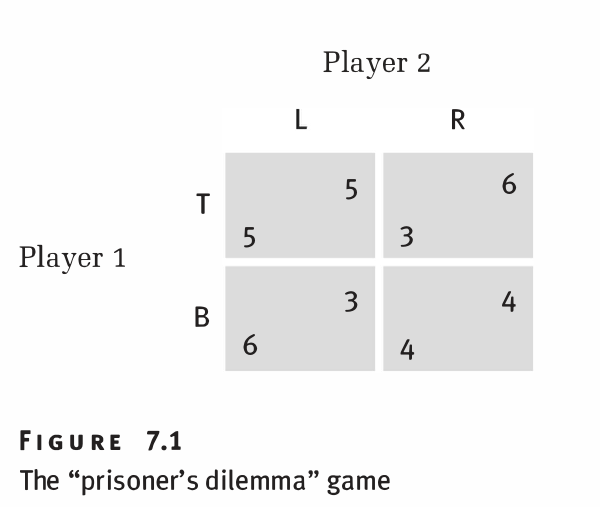
\includegraphics[keepaspectratio,alt={Cabral Figure 7.1, the ``prisoner's dilemma'' game: Player 1 chooses T or B, Player 2 chooses L or R; in each cell Player 1's payoff is lower left and Player 2's upper right: (T,L) = 5, 5; (T,R) = 3, 6; (B,L) = 6, 3; (B,R) = 4, 4}]{../figures/cabral-7-1.png}}



\emph{Figure 7.1} The ``prisoner's dilemma'' game (p.~160). In each cell, Player 1's payoff is in the lower left corner and Player 2's in the upper right corner.

\end{quote}

